\section{Physikalische Grundlagen}

\subsection{Funktionsweise eines Lasers}

1. Describe the general working principles of a laser. In your answer, explain both the fundamental
physical background and the optical arrangement. If several laser transitions are possible, which
criteria determine the actual output wavelength?

\subsection{Stabilitätskriterium des Resonators}

5. What are the stability conditions of a cavity? To determine the stability range of the concentric
cavity used for second harmonic generation (Sec. 2.3.3), make a plot of g 1 g 2 (see Eq. 2.3.3) as a
function of the mirror spacing L. In your calculation, assume a concentric cavity which consists of
a spherical mirror (R 1 = 100 mm) and a spherical mirror (R 2 = 150 mm). Compare these results
to the stability curve of a hemispherical cavity consisting of a spherical mirror (R 1 = 100 mm) and
a flat mirror.



\subsection{Eigenschaften des Pr:YLF-Lasers}

2. What are the specific characteristics of a Pr:YLF laser, i.e., why is it interesting to use a Pr:YLF
laser compared to other solid state lasers? In your answer, also make a comparison of the Pr:YLF
laser with the ruby laser and the Nd:YAG laser.

\begin{figure}[H]
\begin{center}
  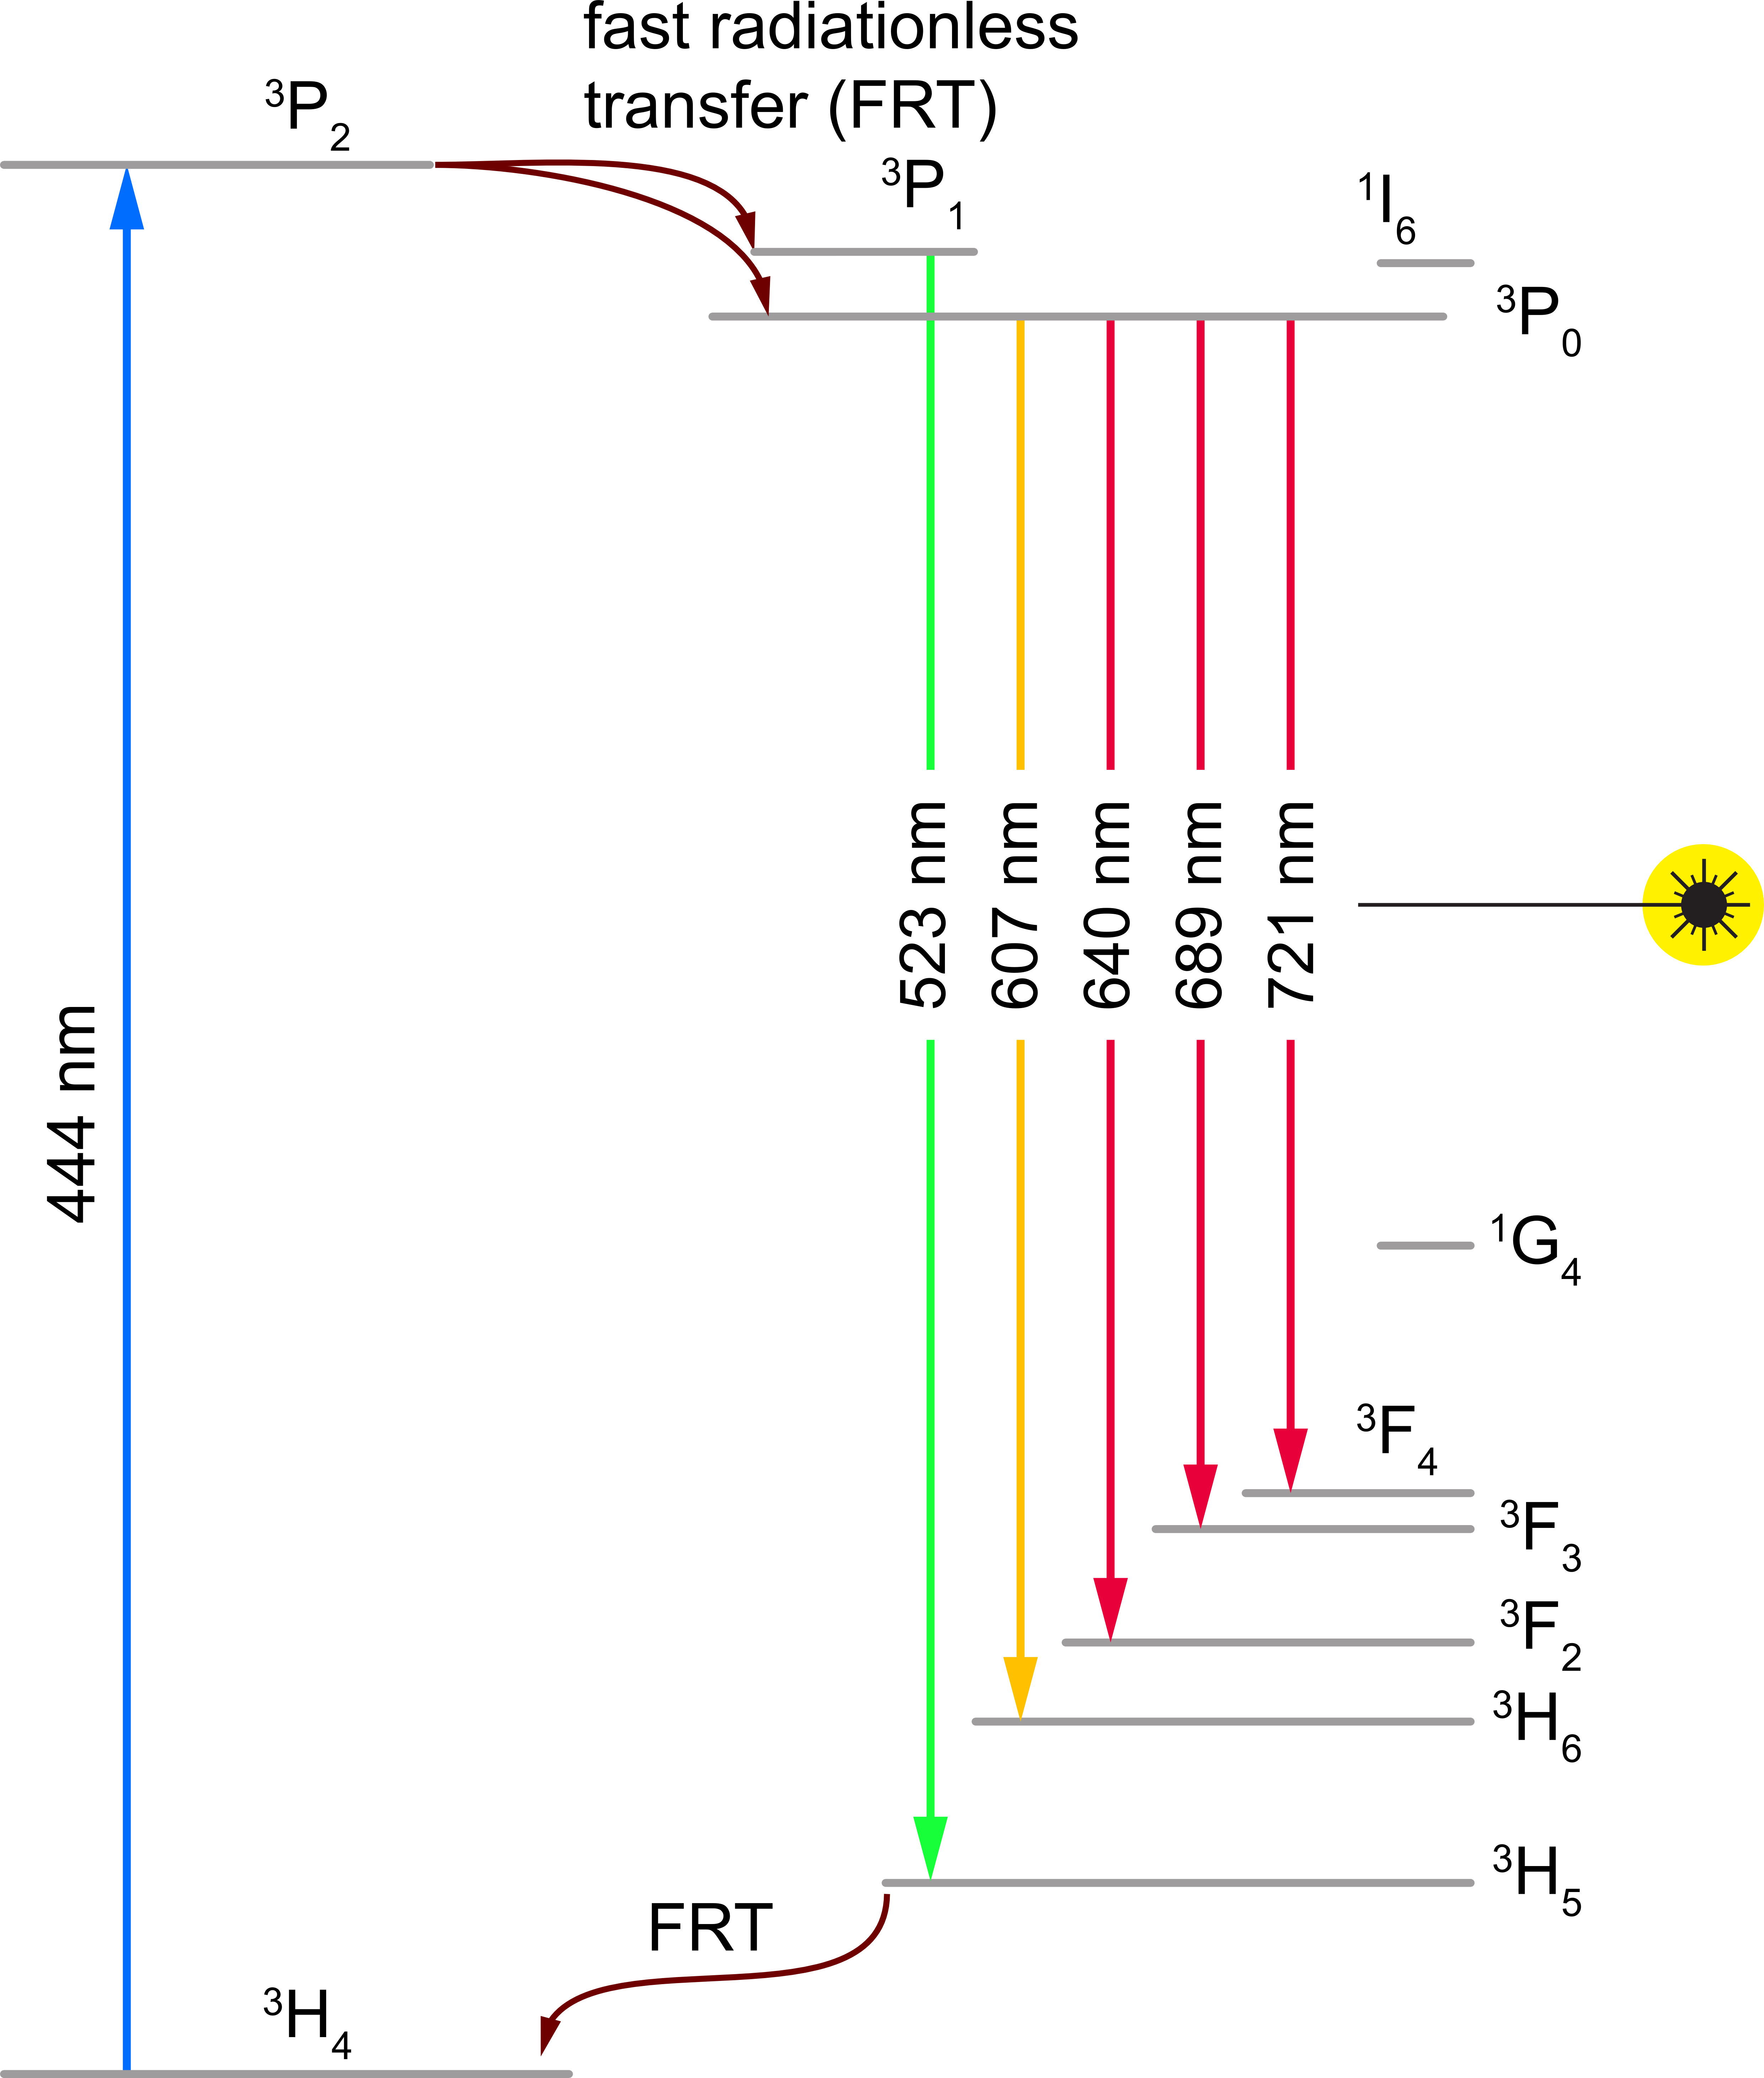
\includegraphics[width=.45\textwidth]{TermschemaPr3+.png}
  \caption{Termschema von Pr$^{3+}$ und relevante Übergänge für den Laserbetrieb
  \cite{Versuchsanleitung}.}
  \label{img:Termschema}
\end{center}
\end{figure}

\subsection{Wellenlängenselektion}


3. Compare the working principles of a birefringent tuner with those of a Littrow prism.


\subsection{Frequenzverdopplung}

4. How does second harmonic generation work and why does it have a low
efficiency?



\subsection{Laserschutzbrillen}

\begin{figure}[H]
\begin{center}
  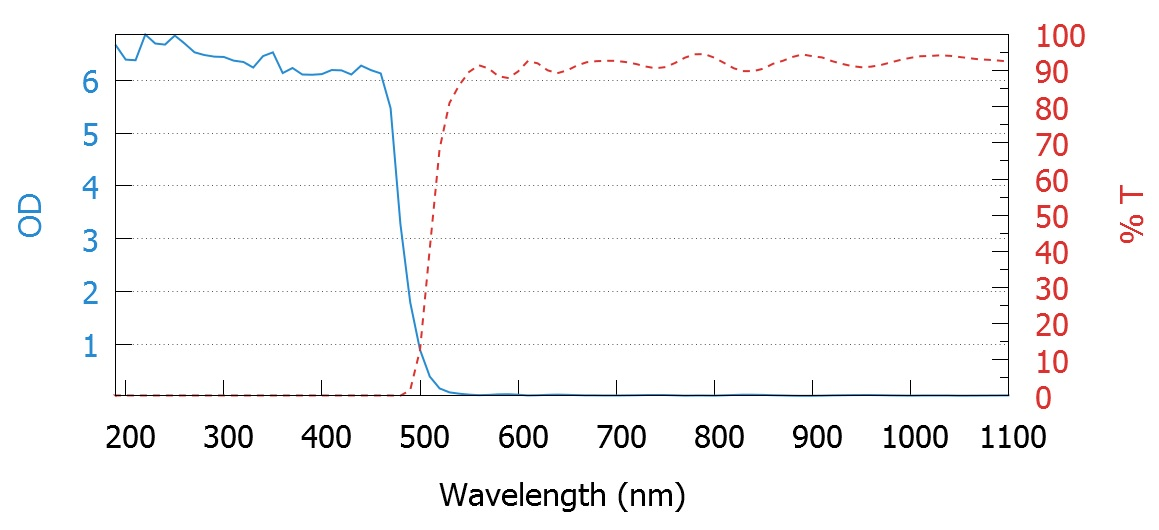
\includegraphics[width=.7\textwidth]{Schutzbrillen.png}
  \caption{Absorptions- (blau)  und Transmissionsspektrum (rot) der im Versuch
  verwendeten Laserschutzbrillen \cite{Versuchsanleitung}.}
  \label{img:Schutzbrillen}
\end{center}
\end{figure}

Abb.~\ref{img:Schutzbrillen} zeigt das Absorptions- und Transmissionsspektrum der
Laserschutzbrillen, die im Versuch verwendet werden.
Strahlung mit Wellenlängen unter 450\,nm wird um einem Faktor von mehr als $10^6$ abgeschwächt und
der starke blaue Pumplaser bei 444\,nm damit fast vollständig blockiert.
Bei Wellenlängen über 500\,nm beginnt eine signifikante Transparenz und über 550\,nm gelangt mehr
als 90\,\% des Lichts durch die Schutzbrillen,
so dass die Linien des Pr:YLF-Lasers beobachtet werden können.

